% CQL vs NYT 4th Down Bot: Agreement with Coaching Decisions
% Replaces: tab:cql-nyt-comparison in section_fourth_down_cql.tex
% Grouped bar chart showing CQL's dominance over NYT Bot

\begin{figure}[htbp]
\centering
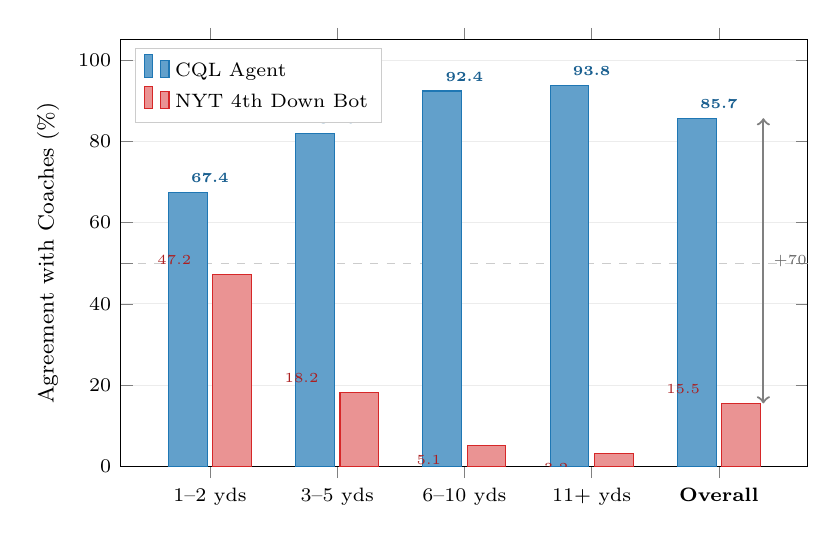
\begin{tikzpicture}
\definecolor{colCQL}{RGB}{31,119,180}
\definecolor{colNYT}{RGB}{214,39,40}

\begin{axis}[
  width=0.85\textwidth,
  height=7cm,
  ybar,
  bar width=14pt,
  ylabel={Agreement with Coaches (\%)},
  ylabel style={font=\footnotesize},
  ymin=0, ymax=105,
  xtick={1,2,3,4,5},
  xticklabels={
    {1--2 yds},
    {3--5 yds},
    {6--10 yds},
    {11+ yds},
    {\textbf{Overall}}
  },
  xticklabel style={font=\scriptsize},
  ytick={0,20,40,60,80,100},
  yticklabel style={font=\scriptsize},
  legend style={at={(0.02,0.98)}, anchor=north west, font=\scriptsize, draw=gray!40, cells={anchor=west}},
  grid=major,
  grid style={gray!15},
  xmajorgrids=false,
  enlarge x limits={abs=0.7},
  extra y ticks={50},
  extra y tick labels={},
  extra y tick style={grid style={black!20, dashed}},
]

% CQL bars
\addplot[fill=colCQL!70, draw=colCQL] coordinates {
  (1, 67.4) (2, 82.0) (3, 92.4) (4, 93.8) (5, 85.7)
};
\addlegendentry{CQL Agent}

% NYT Bot bars
\addplot[fill=colNYT!50, draw=colNYT] coordinates {
  (1, 47.2) (2, 18.2) (3, 5.1) (4, 3.2) (5, 15.5)
};
\addlegendentry{NYT 4th Down Bot}

% Gap annotations
\node[font=\tiny\bfseries, text=colCQL!80!black, anchor=south] at (axis cs:1,67.4) {67.4};
\node[font=\tiny\bfseries, text=colCQL!80!black, anchor=south] at (axis cs:2,82.0) {82.0};
\node[font=\tiny\bfseries, text=colCQL!80!black, anchor=south] at (axis cs:3,92.4) {92.4};
\node[font=\tiny\bfseries, text=colCQL!80!black, anchor=south] at (axis cs:4,93.8) {93.8};
\node[font=\tiny\bfseries, text=colCQL!80!black, anchor=south] at (axis cs:5,85.7) {\textbf{85.7}};

\node[font=\tiny, text=colNYT!80!black, anchor=south] at (axis cs:0.72,47.2) {47.2};
\node[font=\tiny, text=colNYT!80!black, anchor=south] at (axis cs:1.72,18.2) {18.2};
\node[font=\tiny, text=colNYT!80!black, anchor=north] at (axis cs:2.72,5.1) {5.1};
\node[font=\tiny, text=colNYT!80!black, anchor=north] at (axis cs:3.72,3.2) {3.2};
\node[font=\tiny, text=colNYT!80!black, anchor=south] at (axis cs:4.72,15.5) {15.5};

% Gap label for overall
\draw[<->, thick, black!50] (axis cs:5.35,15.5) -- node[right, font=\tiny, text=black!60] {+70.2pp} (axis cs:5.35,85.7);

\end{axis}
\end{tikzpicture}
\caption[CQL vs NYT 4th Down Bot]{CQL vs.\ NYT 4th Down Bot agreement with coaching decisions ($n=5{,}885$ plays, 2024). CQL achieves 85.7\% overall agreement versus NYT's 15.5\%---a +70.2pp advantage. The gap widens with distance: at 11+ yards, CQL agrees with 93.8\% of coaching decisions versus NYT's 3.2\%. CQL learns conservative coaching behavior; NYT optimizes pure expected value.}
\label{fig:cql-vs-nyt-chart}
\end{figure}
